\documentclass[../main/main.tex]{subfiles}

\newdate{date}{20}{12}{2019}


\begin{document}

\chapter{Renormalization group theory. Universality}

\marginpar{ \textbf{Lecture 20.} \\  \displaydate{date}. \\ Compiled:  \today.}

\section{Renormalization group theory (RG)}

Kadanoff's argument for the Ising model allows us to explain the scaling form of the free energy density and of the correlation length near the critical point; in particular, the Kadanoff's block spin transformation justifies the Widom scaling hypothesis and identifies \( \lambda  \) with \( l \). We have obtained the results:
\begin{equation*}
  \begin{cases}
   f_s (t,h) = l^{-d} f_s \qty(t l^{y_t}, h l^{y_h}) \\
   G (\va{r},t,h) = l^{-2(d-y_h)} G \qty(\frac{\va{r}}{l}, t l^{y_t}, h l^{y_h}) \\
   t_l = t l ^{y_t}, \quad h_l = h^{y_h}
  \end{cases}
\end{equation*}
where we did two crucial assumptions:
\begin{enumerate}
\item \( 1^{st} \) assumption:
 \begin{equation*}
  \mathcal{H}_l = \mathcal{H}_\Omega
\end{equation*}
\item \( 2^{nd} \) assumption:
\begin{equation*}
  \begin{cases}
   t_l = t l^{y_t}\\
   h_l = h l^{y_h}
  \end{cases}
\end{equation*}
\end{enumerate}
 \noindent However, as we have seen, the Kadanoff's theory is unable to predict the values of the scaling exponents \( y_t \) and \( y_h \)  (and thus ultimately of the critical exponents), nor can it explain why universality occurs.

 \begin{remark}
 Open problems are: how an iterative procedure of coarse-graining can produce the \( 2^{nd} \) assumption? How this can gives rise to the singular behaviour of \( f_s \)? How can we explain universality of the critical points?
 \end{remark}


We will see that these problems are solved with the introduction of the Renormalization Group (done by K. G. Wilson at the beginning of the '70s), which we will call simply "RG" from now on for the sake of simplicity. The RG is based upon the correct "intuition" of Kadanoff's argument that the coupling constants of a Hamiltonian change if we coarse-grain the system (or in other words we "look" at it on different spatial scales); however, this "intuition" strictly speaking is not correct since we have seen that in Kadanoff's procedure we assume that after the coarse-graining procedure the Hamiltonian of the system has exactly the same form: as we will see, this is not true in general because new terms can appear after we coarse-grain the system.

\subsection{Main goals of RG}
The main goals of the Renormalization Group theory are:
\begin{enumerate}
\item To fornish an algorithm way to perform systematically the coarse graining procedure.

More specifically, the realization of a coarse graining procedure, also called decimation, is like the one introduced by Kadanoff for the Ising model; in general, this procedure must integrate the degrees of freedom of the system on scales of linear dimension \( la \)  which must be much larger than the characteristic microscopic scale \( a \) of the system, but also much smaller than the correlation length \( \xi  \):
\begin{equation*}
  a \ll la \ll \xi
\end{equation*}
 After the decimation, we are left with a new effective Hamiltonian that describes the system at larger length scales. We will see that this is equivalent to find a transformation between the coupling constants \( K \rightarrow K' \).

\item Identify the origin of the critical behaviour and explain universality.

The coarse graining procedure will give rise to a system with \( \xi_l = \xi /l \),
this means that the new correlation length is smaller than the original one, so our system is farther from criticality after the decimation.

\end{enumerate}

To make an example, suppose we are given a generic Hamiltonian \( \mathcal{H} = \mathcal{H} ([K]) \) which depends on an arbitrary number of coupling constants
\( [K] = \va{K} = \qty(K_1,K_2,\dots K_n)  \) (in the case of an Ising model with nearest-neighbour interaction and an external field there are only two coupling constants, \( K = K_1 \) and \( h = K_2 \)).

Let us suppose we apply a coarse-graining procedure, in which we integrate the degree of freedom within distance \( l \) with \( a \le la \le L \).
For what we have just stated, the action of the RG can be expressed as a transformation of the coupling constants:
\begin{empheq}[box=\myyellowbox]{equation}
  [K'] = \mathcal{R}_l [K], \quad l > 1
  \label{eq:20_1}
\end{empheq}
where \( \mathcal{R}_l \) is called \emph{RG transformation},  while this last equation is referred to as \emph{recursive relation}.


\subsubsection{Properties of \( \pmb{\mathcal{R}_l} \)}

We suppose that the function \( \mathcal{R}_l \) satisfy the following properties:

\begin{enumerate}
\item \( \mathcal{R}_l \) is \textbf{analytic} (sum of a finite number of degrees of freedom, no matter how complicated it may be).


\item The set of  transformations \( \mathcal{R}_l \) forms a \textbf{semigroup}, because if we subsequently apply two transformations \(\mathcal{R}_{l_1}  \) and \(\mathcal{R}_{l_2}  \) on two different length scales \( l_1 \)  and \( l_2 \) we have:
\begin{equation*}
  \begin{cases}
   [K'] = \mathcal{R}_{l_1} [K] \\
  [K''] = \mathcal{R}_{l_2} [K'] = \mathcal{R}_{l_2} \circ \mathcal{R}_{l_1} [K]
  \end{cases}
\end{equation*}
Hence, we have the relation
\begin{equation}
  \mathcal{R}_{l_2 l_1} [K] = \mathcal{R}_{l_2} \circ \mathcal{R}_{l_1} [K]
\end{equation}

\begin{remark}
Note that it is a \emph{semigroup} and not a \emph{group}, since in general does not exist the inverse transformation; in fact, we should have always \( l>1 \).
\end{remark}

There is no general way to construct the function \(  \mathcal{R}_l  \): depending on the system and on the case considered we can choose different ways to carry out the decimation, and in general (as we will see) for a given system many different RG transformations can be built. In general such procedures can be done either in coordinate space (real space Renormalization Group) or in Fourier space (momentum shell Renormalization Group).

In terms of the coupling constants \( [K] \) the partition function of the original system is:
\begin{equation*}
  Z_N [K] = \Tr e^{-\beta \mathcal{H}[K]}
\end{equation*}
while the free energy density is
 \begin{equation*}
   f_N [K] = - \frac{k_B T}{N} \log{Z_N [K]}
 \end{equation*}

 Now, if the RG transformation integrates the degrees of freedom on the spatial scale \( la \)  then the number of degrees of freedom will decrease by a factor \( l^d \), if \( d \) is the dimensionality of the system; in other words, after the RG transformation \( \mathcal{R}_l \), the number \( N \) of degrees of freedom is reduced by
\begin{equation*}
  N_l = \frac{N}{l^d}
\end{equation*}

\item The new hamiltonian \( \mathcal{H}_l [K'] \) can be (and in general it is) different from the previous one \( \mathcal{H} [K] \) (this is the main difference with the Kadanoff's theory), but the effective Hamiltonian \(  \mathcal{H}_l [K']\)  must have the same symmetry properties of the original one!

This means (and this is the great improvement with respect to Kadanoff's argument) that the decimation can make some new terms appear in the coarse-grained Hamiltonian, as long as they respect the same symmetries of the original system. In other words, if \( K_m=0 \)  in \( \mathcal{H}_N \)  but its relative term is allowed by the symmetry group of \( \mathcal{H}_N \)  itself, then we can have \( K_m' \neq 0 \) in \( \mathcal{H}_{N'}' \).

For example, if we start from
\begin{equation*}
  \mathcal{H}_N = N K_0 + K_2 \sum_{ij}^{} S_i S_j
\end{equation*}
if the term \( K_3 \) is not allowed by the symmetry group of \( \mathcal{H}_N \), we cannot produce
\begin{equation*}
  \mathcal{H}_{N'}' = N' K_0' + K_1' \sum_{I}^{} S_I + K_2' \sum_{IJ}^{} S_I S_J
  + \mathcolorbox{red!20}{ K_3' \sum_{IJK}^{} S_I S_J S_K}
\end{equation*}

\item The invariance condition is not in \( \mathcal{H} \) (as in Kadanoff's theory) but in \( Z \); hence, the coarse-graining procedure (decimation) leaves invariant the partition function instead of the Hamiltonian:
\begin{equation}
  Z_{N'} [K'] = Z_N [K]
  \label{eq:20_2}
\end{equation}
this invariance condition has a consequence on the free-energy:
  \begin{equation*}
  f_N [K]  \simeq \frac{1}{N} \log{Z_N [K]} \simeq \frac{l^d}{l^d N} \log{Z_{N'}[K']} \simeq l^{-d} \frac{1}{N'} \log{Z_{N'}} [K']
\end{equation*}
where \( N' = N/l^d \).
Hence,
\begin{equation}
  f [K] \propto l^{-d} f [K']
\end{equation}
which is the scaling form of the free energy density as obtained by Kadanoff.

\end{enumerate}



\subsection{Singular behaviour in RG}

We have stated that the RG transformations \( \mathcal{R}_l \) are analytic, hence a single \( \mathcal{R}_l \) involves the integration of a finite number of dregrees of freedom and the free energy cannot develop the singularity behaviour we are looking for; so, we might ask: where does the singular behaviour of a system near a critical point come from? This occurs in the thermodynamic limit, which in this case is obtained when we apply the RG transformation an infinite number of times. Indeed, in order to integrate a thermodynamic number of degrees of freedoms, one has to apply an infinite number of RG transformations.

In general, after the \( n \)-th iteration of the RG, the coarse-graining length of the system will be \( l \rightarrow l^n \) and the coupling constants \( [K] \rightarrow [K^{(n)}] \).
As \( n \) increases the "vector" of coupling constants describes a "trajectory" in the space of all the possible coupling constants \( [K] \), often called \textbf{Hamiltonian space}, or theory space;
by varying the initial conditions, namely different initial Hamiltonians, one obtains a
\textbf{flux of trajectories} (i.e. the set of all the trajectories that start from different initial conditions).
In general, these trajectories can form strange attractors or complex limit cycles; however, it is almost always found that they are simply attracted towards or ejected from \textbf{fixed points} (cases where this doesn't occur are really exotic), so in the following we will assume that the flux of trajectories only exhibits fixed points.

The study of the properties of the flux of trajectories near these fixed points is crucial, since as we will see it is that that will allow us to actually explain universality and predict the values of the critical exponents (the scaling behaviour introduced by Widom is related to the behaviour of the trajectories close to some fixed points). We therefore proceed to study such points.







 \subsection{Zoology of the fixed points}
 Suppose we know \( \mathcal{R}_{l} \). If \( [K^*] \) is a fixed point of the flux of trajectories, by definition we have:
 \begin{equation}
    \mathcal{R}_l [K^*] = [K^*]
 \end{equation}
 Then, in general from the Hamiltonian of a system we can determine the correlation length \( \xi  \), and if \( [K'] = \mathcal{R}_l [K] \)  we know that:
\begin{equation*}
  \xi [K'] = \frac{\xi [K]}{l} \equiv \xi _l
\end{equation*}
Therefore for a fixed point we have:
\begin{equation}
  \xi [K^*] = \frac{\xi [K^*]}{l}
\end{equation}
which implies two cases:
\begin{equation}
  \xi [K^*] =
  \begin{cases}
   0 & \text{trivial}\\
   \infty & \text{critical}
  \end{cases}
\end{equation}
A fixed point with \( \xi = \infty  \) is called \emph{critical}, while if \( \xi =0 \) \emph{trivial}. Clearly, every fixed point \( [K^*] \)  can have its own \textbf{basin of attraction}, i.e. a set of points \( \{ [K] \}   \) that under the action of the flux of trajectories tend to \( [K^*] \):
\begin{equation}
  \mathcal{R}_l^{(n)} [K] \overset{n \rightarrow \infty }{\longrightarrow} [K^*]
\end{equation}
An important result concerning the basin of attraction of critical fixed points is the following:


\begin{theorem}{}{}
All the points \([K]  \) belonging to a basin of attraction of a critical fixed point have the correlation length \( \xi = \infty  \).
\end{theorem}
\begin{proof}
  Call \( [K] \) the initial set of coupling constants, after \( n \)  iterations of the RG the correlation length of the system will be such that:
\begin{equation*}
  \xi [K] = l \xi [K^{(1)}] = \dots =l^n \xi [ K^{(n)}] \quad \Rightarrow \xi [K] = l^n \xi [ K^{(n)}]
\end{equation*}
If we now take the limit \( n \rightarrow \infty  \)  the right hand side diverges if \( K^{(n)} \rightarrow K^* \), i.e. if \( [K] \)  belongs to the basin of attraction of \( [K^*] \).
Hence, \( \xi [K^*] = \infty  \), implies
\begin{equation*}
  \Rightarrow \xi [K] = l^n \xi [K^*] = \infty
\end{equation*}
Therefore, we have \( \xi [K] = \infty  \).

\end{proof}

The set of \( [K] \) that forms the basin of attraction of a critical fixed point is also called \textbf{critical manifold}.

\subsubsection{Universality}

All the critical models that belong to the critical manifold, have the same critical behaviour of the corresponding critical fixed point. Hence, we want to study the behaviour of \( \mathcal{R}_l \) close to the fixed points.

 We can argue that the fact that all the points of a critical manifold flow towards the same fixed point (i.e. the same Hamiltonian) is the basic mechanism on which universality is based upon, but this is by no means a complete explanation, since universality involves the behaviour of systems near a critical point and we still have said nothing about that. We can however note the following fact: starting from any point in Hamiltonian space, iterating the RG transformation and identifying the fixed point towards which the system flows, the phase of the original point in Hamiltonian space (i.e. in the phase diagram) will be described by this fixed point. Therefore, every phase of the system is "represented" by a fixed point of the flux of trajectories.


As we will later see, critical fixed points describe the singular critical behaviour while trivial fixed points are related to the bulk phases of the system: therefore, the knowledge of the location and nature of the fixed points of the flux of trajectories can give us hints on the structure of the phase diagram of the system, and the behaviour of the flow near critical fixed points allows us to calculate the values of the critical exponents.




\subsection{Linearization of RG close to the fixed points and critical exponents}

In order to study the behaviour of the flux of trajectories near a fixed point \( [K^*] \) of \( \mathcal{R}_l \), let us take a slight perturbation from it, namely we set:
\begin{equation}
  \va{K} = \va{K}^* + \delta \va{K}
\end{equation}
where \( \delta \va{K} \) is a small displacement. Applying the RG transformation, in components we will have:
\begin{equation*}
  K'_j = (\mathcal{R}_l)_j (\va{K}^*+ \delta \va{K} )_j
= K^*_j + \sum_{i}^{} \eval{\qty(\pdv{K_j'}{K_i} )}_{\va{K}^*} \delta K_i + O \qty(\delta K_i^2)
\end{equation*}
Neglecting all the terms beyond the linear ones, we can write the action of the linearised RG transformation in terms of the displacements \( \delta \va{K} \) and
\( \delta \va{K}' \) as:
\begin{equation}
  \delta \va{K}' = \bar{\pi } \delta \va{K}
\end{equation}
where
\begin{equation}
  \qty(\bar{\pi } )_{ij} = \eval{\qty(\pdv{K_j'}{K_i} )}_{\va{K}^*}
\end{equation}
Of course \( \bar{\pi } \) is a square matrix, but:
\begin{enumerate}
\item \( \bar{\pi }  \) is in general not symmetric, one has to distinguish between left and right eigenvectors;
\item \( \bar{\pi }  \) it is not always diagonalizable or sometimes its eigenvalues can be complex. For most of the physical system, however, \( \bar{\pi }  \) can be diagonalized and the eigenvalues are real.
\end{enumerate}
However, we suppose \( \bar{\pi } \) to be symmetric (which, as before, is almost always the case) so that it can be diagonalized. If we call \( \lambda _l^{(\sigma)} \) and \( \va{e}^{(\sigma )} \) the \( \sigma  \)-th  eigenvalue and relative eigenvector of \( \bar{\pi }^{(l)} \)  (where we are explicitly writing the length scale of the decimation), in components the action \(\bar{\pi }^{(l)}  \) will be:
\begin{equation}
  \Rightarrow \bar{\pi }^{(l)}_{ij} \va{e}^{(\sigma )}_j = \lambda _l^{(\sigma )} \va{e}_i ^{(\sigma )}
\end{equation}
this is the eigenvalue equation. From the semigroup property of the RG transformation \( \mathcal{R}_l \), we have:
\begin{equation*}
  \bar{\pi }^{(l)} \bar{\pi }^{(l')} = \bar{\pi }^{(ll')}
\end{equation*}
Hence, we have:
\begin{equation}
  \lambda _l^{(\sigma )} \lambda _{l'}^{(\sigma )} =  \lambda _{ll'}^{(\sigma )}
  \label{eq:20_3}
\end{equation}
This is a functional equation which can be solved in the following way:  if we write the eigenvalues explicitly as functions of \( l \), namely \( \lambda _l^{(\sigma )}= \lambda^{(\sigma )}  (l)\), then differentiating with respect to \( l' \):
\begin{equation*}
   \lambda ^{(\sigma )}(l )\lambda '^{(\sigma )}(l')=\ell \lambda '^{(\sigma )}(l l ')
\end{equation*}
where with \( \lambda ' \)  we mean that \( \lambda  \)  has been differentiated with respect to its argument. Setting now \( l'=1 \)  and defining \( \lambda'^{(\sigma )} (1) = y_\sigma \)  we get:
\begin{equation*}
  \frac{\lambda'^{(\sigma )} (l)}{\lambda^\sigma (l)} = \frac{ y_\sigma}{l}
\end{equation*}
which is easily solved to give:
\begin{equation}
   \lambda _{l}^{(\sigma )} = l^{y_\sigma}
\end{equation}
where, as we have defined it, \( y_\sigma \) is a number (to be determined) independent of \( l \)  (is the critical exponent). To see how \( \delta \va{K} \) changes under the action of the linearized transformation  \( \bar{\pi }  \) let us find out how its components along the directions determined by the eigenvectors \( \va{e}^{(\sigma )} \) change.  In other words, let us expand \( \delta \va{K} \) in terms of \( \va{e}^{(\sigma )} \) (that is a complete orthonormal base):
\begin{equation}
  \delta \va{K} = \sum_{\sigma }^{} a^{(\sigma )} \va{e}^{(\sigma )}, \qquad a^{(\sigma )} = \va{e}^{(\sigma )} \vdot \delta \va{K}
\end{equation}
and applying \( \bar{\pi }^{(l)}  \):
\begin{equation}
  \delta \va{K}' = \bar{\pi } \delta \va{K} = \sum_{\sigma }^{} a^{(\sigma )} \bar{\pi } \qty(\va{e}^{(\sigma )})
  = \sum_{\sigma }^{} a^{(\sigma )} \lambda_l ^{(\sigma )} \va{e}^{(\sigma )}
  \equiv  \sum_{\sigma }^{} a'^{(\sigma )} \va{e}^{(\sigma )}
\end{equation}
where in the last step we have defined the components \( a'^{(\sigma )} \) which is the projection of \( \delta \va{K}' \) along \( \va{e}^{(\sigma )} \).
\begin{remark}
Ortonormality is not always true since in general \( \bar{\pi }  \) is not symmetric!
  \end{remark}

We therefore see that the behaviour of \( \delta \va{K} \)  along the eigenvectors \( \va{e}^{(\sigma )} \)  depends on the magnitudes of the eigenvalues \( \lambda_l^{(\sigma )} \): some components of \( \delta \va{K} \) grow under the action of \( \bar{\pi }  \) while some others shrink. In particular, if we order the eigenvalues in descending order
\begin{equation*}
  \abs{\va{\lambda }_1} \ge \abs{\va{\lambda }_2} \ge \abs{\va{\lambda }_3} \ge \dots \ge \abs{\va{\lambda }_{\sigma}}
\end{equation*}
we can distinguish three cases:
\begin{enumerate}
\item case \( \abs{\lambda_l ^{(\sigma )}} > 1 \) (i.e. \( y^\sigma > 0\)): implies that \( a^{(\sigma )} \) grows under \( \bar{\pi }  \). These are called \textbf{relevant} eigenvalues/eigenvectors;

\item case \( \abs{\lambda_l ^{(\sigma )}} < 1 \) (i.e. \( y^\sigma < 0\)): implies that \( a^{(\sigma )} \) decreases under \( \bar{\pi }  \). These are called \textbf{irrelevant} eigenvalues/eigenvectors;

\item case \( \abs{\lambda_l ^{(\sigma )}} = 1 \) (i.e. \( y^\sigma =  0\)): implies that \( a^{(\sigma )} \) remains constant under \( \bar{\pi }  \) (its behaviour can depend on the higher orders in the expansion that we have neglected). These are called \textbf{marginal} eigenvalues/eigenvectors.
\end{enumerate}

The above analysis implies that: starting from a point close to a critical fixed point \( [K^*] \) (but not on the critical manifold), the trajectory will abandon \( [K^*] \) along the relevant directions whereas it will approach \( [K^*] \) along the irrelevant directions. Hence, we have that:
\begin{itemize}
\item The \emph{irrelevant} eigenvectors form the local basis of the basin of attraction of \( [K^*] \). Hence, the number of irrelevant directions of a fixed point is equal to the dimension of its critical manifold.
\item The \emph{relevant} eigenvectors form a sub-space complementar to the basin of attraction of codimension \( C \). Hence, the number of relevant directions is equal to its codimension.
\end{itemize}

\begin{remark}
Let us note that the eigenvalues, and their possible relevance, depend on the matrix \( \bar{\pi }  \), which in turn depends on the fixed point considered \( [K^*] \): this means that the terms "relevant", "irrelevant" or "marginal" must always be specified with respect to the particular fixed point considered.
\end{remark}


\section{The origins of scaling and critical behaviour}
Let us consider a fixed point of the flux of trajectories of a generic system, and assume that it has two relevant directions corresponding to the coupling constants that for simplicity we defined as
\begin{equation*}
  K_1 \rightarrow K_1 (T) = T, \qquad K_2 \rightarrow K_2 (H) = H
\end{equation*}
where \( T \) is the temperature and \( H \) is the external field.  We suppose that
\( T \) and \( H \)  are transformed under the RG such that:
\begin{equation*}
  T' = \mathcal{R}_l ^T (T,H), \qquad H' = \mathcal{R}_l ^H (T,H)
\end{equation*}
where \( \mathcal{R}_l ^T  \) and \( \mathcal{R}_l ^H  \) are analytic functions given by the coarse graining procedure.  The fixed points \( \va{K}^* = (T^*,H^*) \)  of the flux of trajectories will be given by the solutions of:
\begin{equation*}
  \begin{cases}
   T^* = \mathcal{R}_l ^T (T^*,H^*)\\
   H^* = \mathcal{R}_l ^H (T^*,H^*)
  \end{cases}
\end{equation*}
with the correlation length that diverges, i.e. \( \xi (T^*,H^*) = \infty  \).
Linearising the transformation around the fixed point \( (T^*,H^*) \), in terms of the reduced variables (for standard magnetic systems \( H^*=0 \) )
\begin{equation*}
  t = \frac{(T-T^*)}{T^*}, \qquad h = \frac{(H-H^*)}{H^*}
\end{equation*}
we have:
\begin{equation}
  \begin{pmatrix}
  t' \\
  h'
  \end{pmatrix}
  = \bar{\pi }
  \begin{pmatrix}
  t \\
  h
  \end{pmatrix}
\end{equation}
where:
\begin{equation}
  \bar{\pi } =
  \begin{pmatrix}
    \partial{\mathcal{R}_l^T} / \partial{T}  & \partial{\mathcal{R}_l^T} / \partial{H} \\
     \partial{\mathcal{R}_l^H} / \partial{T}  &\partial{\mathcal{R}_l^H} / \partial{H}
  \end{pmatrix}_{T^*,H^*}
\end{equation}
\begin{remark}
In this case \( \delta \va{K}  = (t,h) \).
\end{remark}

In general the eigenvectors \( \va{e}^{(\sigma )} \) are linear combinations of \( t \) and \( h \). When \( \bar{\pi }  \) can be diagonalized, \( t \) and \( h \) are not "mixed-up" by the transformation. Hence, as previously stated, we suppose \( \bar{\pi }  \) to be diagonalizable. We therefore write its eigenvalues as:
\begin{equation}
  \lambda _l ^{(t)} = l^{y_t}, \quad \lambda _l^{(h)} = l ^{y_h}
\end{equation}
This way we can write the linear transformation as:
\begin{equation}
  \begin{pmatrix}
  t' \\
  h'
  \end{pmatrix}
  =
  \begin{pmatrix}
  \lambda _l^{(t)}   & 0 \\
    0 & \lambda _l^{(h)}
  \end{pmatrix}
  \begin{pmatrix}
  t \\
  h
  \end{pmatrix} \quad \Rightarrow \quad
  \begin{pmatrix}
  t' \\
  h'
  \end{pmatrix}
  =
  \begin{pmatrix}
  l^{y_t} t \\
  l ^{y_h} h
  \end{pmatrix}
\end{equation}
After \( n \) iterations we will have:
\begin{equation}
  \begin{cases}
   t^{(n)} = \qty(l^{y_t})^n t  \\
  h^{(n)} = \qty(l^{y_h})^n h
  \end{cases}
\end{equation}
On the other hand, since in general we know that
\begin{equation*}
  \xi' \equiv \xi (t',h') = \frac{\xi (t,h)}{l}
\end{equation*}
after \( n \) iterations we have
\begin{equation}
  \xi (t,h) = l^n \xi \qty(l^{n y_t} t, l^{n y_h} h)
\end{equation}
This is the scaling law of the correlation length. From this we can determine the critical exponent \( \nu  \).  In fact, setting \( h=0 \) \( (H=H^*) \) for simplicity, we have
\begin{equation*}
  \xi (t,0) = l^n \xi \qty(l^{n y_t} t , 0)
\end{equation*}
Since \( l \) is arbitrary, choosing it  so that \( l^{n y_t} t = b \gg 1\), with \( b \)  a positive real number (\( b \in \R^+ \), \( l \) is not an integer any more), we have:
\begin{equation*}
  l^n = \qty(\frac{b}{t})^{1/y_t} \quad   \Rightarrow \xi (t) = \qty(\frac{t}{b})^{-1/y_t} \xi (b,0)
\end{equation*}
Since for \( t \rightarrow 0 \) in general \( \xi \sim t^{-\nu } \), we get:
\begin{equation}
  \nu = \frac{1}{y_t}
\end{equation}
This is an extremely important result! In fact, we see that once the RG transformation \( \mathcal{R_l} \) is known, \( y_t \) is straightforward to compute as:
\begin{equation*}
  y_t  = \frac{ \log{\lambda _l^{(t)}}}{\log{l} }
\end{equation*}
and so we are actually able to calculate \( \nu  \) and predict its value! We can do even something more (including giving \( y_h \) a meaning) from the scaling law of the free energy density. After \( n \) iterations of the RG we have:
\begin{equation}
f_s (t,h)  = l^{-d} f_s (t',h') = l^{-nd} f_s (t^{(n)},h^{(n)})
 = l^{-nd} f_s \qty(l^{n y_t}t, l^{n y_h}h)
\end{equation}
and choosing again \( l \) so that  \( l^{n y_t} t= b^{y_t} \), then:
\begin{equation*}
  f_s (t,h) = t^{d/y_t} b^{-d} f_s \qty(b^{y_t}, \frac{b^{y_h}h}{t^{y_h/y_t}})
\end{equation*}
Comparing this to what we have seen in Eq.\eqref{eq:19_13} we get:
\begin{equation}
  \begin{cases}
   2 - \alpha = d \nu = \frac{d}{y_t}\\
   \Delta = \frac{y_h}{y_t}
  \end{cases}
\end{equation}
where \( y_h \) and \( y_t \) can be computed as
\begin{equation}
  y_t  = \frac{\log{\lambda _l^{(t)}}}{\log{l} }, \qquad y_h = \frac{\log{\lambda _l^{(h)}}}{\log{l} }
\end{equation}
Hence, we have all we need for the computation!



\section{Real space renormalization group (RSRG)}
We now want to see how we can build the RG transformation \( \mathcal{R}_l \) from the coarse graining procedure.
Let us start from the most general form of the Ising model where \( \sigma _i = \pm 1 \) and the two body interaction is
\begin{equation}
  w (\sigma _i, \sigma _j) = - \hat{g} - \frac{\hat{h} }{z} (\sigma _i + \sigma _j) - \hat{K} \sigma _i \sigma _j
\end{equation}
where \( z \) is the coordination number. The Hamiltonian of such a system is:
\begin{equation}
  Z = \sum_{\{ \sigma  \}  }^{}  e^{\sum_{\expval{ij} }^{}  w (\sigma _i, \sigma _j)}
\end{equation}
Let us consider the one-dimensional case \( d=1 \)  with nearest-neighbour interaction and periodic boundary conditions without any external field \( (H=0) \), as in Figure \ref{fig:20_4}.

\begin{figure}[h!]
\centering
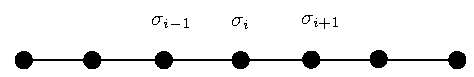
\includegraphics[width=0.6\textwidth]{../lessons/20_image/4.pdf}
\caption{\label{fig:20_4} One-dimensional Ising model.}
\end{figure}

The idea of the renormalization group is to perform an integration over some degrees of freedom and obtain a new partition function with \( N/l^d \) spins but of the same form of the one describing the original system with \( N \) spins.

There are many ways to perform this partial integration. Here we consider the \emph{decimation} procedure with \( l=2 \).

\subsection{Ising \( \pmb{d=1} \), RSRG with \( \pmb{l=2} \).}
A coarse graining of \( l=2  \) can be obtained for instance by summing over the spins positioned at the \emph{even} sites. Before doing this sum it is convenient to rename the even spins \( \sigma _{2i} \) as \( S_i \) and the odd spins (the ones that will survive) \( \sigma _{2i+1} \) as \( \sigma _i' \).

In this way the sum \( \sum_{\{ \sigma  \}  }^{}   \) can be partitioned as \( \sum_{\{ \sigma _i' \}  }^{} \sum_{\{ S_i \}  }^{}     \) where now we have \( i=1,\dots,N/2 \). Hence, the partition function becomes
\begin{equation}
  Z_N(g,k,h) = \sum_{\{ \sigma _i \}_i^N  }^{}  e^{\sum_{i}^{}  w (\sigma _i, \sigma _{i+1})}
  = \sum_{\{ \sigma _i' \}_1^{N/2}  }^{} \sum_{\{ S_i \}_1^{N/2}  }^{}
  e^{\sum_{i=1}^{N/2} \qty[w(\sigma _i',S_i) + w(S_i, \sigma _{i+1}')]  }
  \label{eq:20_6}
\end{equation}
Bringing the summation out of the exponential, we obtain:
\begin{equation*}
  Z_N = \sum_{\{ \sigma _i' \}_1^{N/2}} \prod_{i=1}^{N/2}  \qty(  \sum_{  S_i=\pm 1  }^{}  e^{ \qty[ w(\sigma _i',S_i) + w(S_i, \sigma _{i+1}') ]  }  )
\end{equation*}
Let us note that:
\begin{equation*}
   \sum_{  S_i=\pm 1  }^{}  e^{ \qty[ w(\sigma _i',S_i) + w(S_i, \sigma _{i+1}') ]  }
   = f (\sigma _i', \sigma _{i+1}')
\end{equation*}
If we can write \(  f (\sigma _i', \sigma _{i+1}') \) as an exponential
\( \exp [ w' (\sigma _i', \sigma _{i+1}')]  \), we obtain:
\begin{equation}
  Z_N (g,h,k) = \sum_{\{ \sigma _i' \}_1^{N/2}}  e^{\sum_{i=1}^{N/2}  w' (\sigma _i', \sigma _{i+1}') }
\end{equation}
It has a similar form as the original one (Eq.\eqref{eq:20_6}) but with \( N/2 \) spins.
Supposing that also \( w' (\sigma _i', \sigma _{i+1}')  \) can be written as
\begin{equation*}
  g' + \frac{h'}{z} (\sigma _i' + \sigma _{i+1}') + K' \sigma _i' \sigma _{i+1}'
\end{equation*}
we have
\begin{equation}
  Z_N (g,h,K) = Z_{N/2} (g',h',K')
\end{equation}
as requested by the renormalization group.
In order to find \( g',h',K' \) as a function of \( g,h,K \), we should satisfy the relation
\begin{equation}
  e^{ g' + \frac{h'}{2} (\sigma _i' + \sigma _{i+1}') + K' \sigma _i' \sigma _{i+1}' }
  = \sum_{S_i = \pm 1}^{}  e^{ \overbrace{g + \frac{h}{2}(\sigma _i' + S_i) + K \sigma _i' S_i}^{w(\sigma _i',S_i)}  + \overbrace{g + \frac{h}{2} (S_i + \sigma _{i+1}') + K S_i \sigma _{i+1}' }^{w(S_i,\sigma _{i+1}')}  }
\end{equation}
for all values of the pair \( (\sigma _i',\sigma _{i+1}') \).
\begin{remark}
Remind that the coordination number is \( z=2d \) for an hypercubic lattice; in this case we have \( d=1 \), hence \( z=2 \).
\end{remark}
For simplicity let us consider
\begin{equation}
  \begin{cases}
   x \equiv e^K \,\,\,, \quad y \equiv e^h\,\,\,, \quad  z \equiv e^g \\
   x' \equiv e^{K'}, \quad  y' \equiv e^{h'}, \quad  z' \equiv e^{g'}
  \end{cases}
\end{equation}
Hence, the previous condition becomes
\begin{equation*}
  z' {y'}^{\qty(\frac{\sigma _i'+\sigma _{i+1}'}{2}) } {x'}^{\sigma _i'\sigma _{i+1}'}
  = \sum_{S_i = \pm 1}^{} z^2 y^{\qty(\frac{\sigma _i' +S_i}{2}) } x^{\sigma _i' S_i} y^{ \qty(\frac{S_i + \sigma _{i+1}}{2})} x^{S_i \sigma _{i+1}}
\end{equation*}
Let us consider all the cases for different values of \( \sigma _i' \) and \( \sigma _{i+1}' \), we obtain three independent equations and three variables:
\begin{itemize}
\item Case \( \sigma _i'=+1 \) and \( \sigma _{i+1}'=+1 \):
\begin{equation}
  z'y'x' = z^2 y (x^2y+x^{-2}y^{-1})
  \label{eq:20_7}
\end{equation}

\item Case \( \sigma _i'=-1 \) and \( \sigma _{i+1}'=-1 \):
\begin{equation}
  z'{y'}^{-1}x' = z^2 y^{-1} (x^{-2} y+x^{2}y^{-1})
  \label{eq:20_8}
\end{equation}

\item Case \( \sigma _i'=+1 \) and \( \sigma _{i+1}'=-1 \), or \( \sigma _i'=-1 \) and \( \sigma _{i+1}'=+1 \):
\begin{equation}
  z'{x'}^{-1} = z^2 (y+y^{-1})
  \label{eq:20_9}
\end{equation}
in the two cases the relation obtained is the same.
\end{itemize}
Now, we rearrange these independent equations in the following way:

\begin{itemize}
\item By multuplying Eq.\eqref{eq:20_7}\( \times \)\eqref{eq:20_8}\( \times 2 \vdot   \)\eqref{eq:20_9} we obtain:
\begin{equation*}
  {z'}^4 = z^8 \qty( y + y^{-1})^2 \qty( x^2y + x^{-2}y^{-1}) \qty( x^{-2}y + x^2 y^{-1})
\end{equation*}
\item By dividing Eq.\eqref{eq:20_7}/\eqref{eq:20_8} we obtain:
\begin{equation*}
  {y'}^2 = y^2 \frac{x^2y + x^{-2}y^{-1}}{x^{-2}y+x^2y^{-1}}
\end{equation*}

\item By multiplying and dividing the three equations as (\eqref{eq:20_7}\( \times \)\eqref{eq:20_8})/(\( 2 \vdot \)\eqref{eq:20_9}), we obtain
\begin{equation*}
  {x'}^4 = \frac{\qty(x^2 y + x^{-2} y^{-1})\qty(x^{-2} y + x^2 y^{-1})  }{ \qty(y + y^{-1})^2 }
\end{equation*}

\end{itemize}

Let us note that \( g \) and \( g' \) are constant factors of the partition function \( Z \) and can be absorbed by a shift in the free energies.
Moreover \( g \) (i.e. \( z \equiv e^g \)) does not enter in the expression of \( h' \) and \( K' \); the two relevant renormalization equations are the ones for \( x' \) and \( y' \):
\begin{equation*}
  \begin{cases}
   {y'}^2 = y^2 \frac{x^2y + x^{-2}y^{-1}}{x^{-2}y+x^2y^{-1}} \\
   {x'}^4 = \frac{\qty(x^2 y + x^{-2} y^{-1})\qty(x^{-2} y + x^2 y^{-1})  }{ \qty(y + y^{-1})^2 }
  \end{cases}
\end{equation*}
Taking the logarithm of these equations we obtain:
\begin{equation}
  \begin{cases}
   2h' = 2h + \log{\qty(e^{2K+h} + e^{-2K-h}) } - \log{ \qty(e^{-2K+h} e^{2K-h}) }  \\
  4K' = \log{ \qty(e^{2K+h}+ e^{-2K-h})} + \log{\qty(e^{-2K+h}+e^{2K-h})} - 2 \log{\qty(e^h + e^{-h})}
  \end{cases}
  \label{eq:20_10}
\end{equation}
Hence, we have obtained the renormalization group transformation
\begin{equation*}
  (h',K') \rightarrow \mathcal{R}_l (h,K)
\end{equation*}
Now, let us look for fixed points \( (h^*,K^*) \); then will we linearized around \( (h^*,K^*) \) and we will find the relevant eigenvalues.

Let us consider for simplicity \( h=0 \), so that \( y \equiv e^h = 1 \). The equations \eqref{eq:20_10} simplify to
\begin{equation*}
  \begin{cases}
   {y'}^2 = \frac{x^2 + x^{-2}}{x^{-2} + x^2}\\
   {x'}^4 = \frac{\qty(x^2 + x^{-2})\qty(x^{-2}+ x^2)  }{4}
  \end{cases}
\end{equation*}
Hence, we have:
\begin{equation}
  \begin{cases}
   y'=1\\
   {x'}^4 = \frac{\qty(x^2 + x^{-2})^2 }{4}
  \end{cases}
\end{equation}
 Therefore, we have that \( K \) is the only variable left because we have obtained \( h'=0 \). By substituting \( x' \equiv e^K \), we have:
\begin{equation*}
   {x'}^4 = \frac{\qty(x^2 + x^{-2})^2 }{4} \quad \Rightarrow e^{4K'} = \qty( \frac{e^{2K} + e^{-2K} }{2} )^2 = \cosh^2 (2K)
\end{equation*}
In conclusion we obtain the RG equation:
\begin{empheq}[box=\myyellowbox]{equation}
  K' = \frac{1}{2} \log{\qty( \cosh (2K)) }
  \label{eq:20_11}
\end{empheq}
By rearranging we have:
\begin{equation*}
  e^{2K'} = \cosh (2K) = 2 \cosh^2 (K) - 1 \quad \Rightarrow e^{2K'} - 1  = 2 \qty( \cosh^2(K) - 1) = 2 \sinh^2 (K)
\end{equation*}
Similarly,
\begin{equation*}
  e^{2K'} + 1 = 2 \cosh^2 (K)
\end{equation*}
Hence,
\begin{equation*}
  \frac{e^{2K'} - 1}{e^{2K'} + 1} = \tanh (K') = \tanh^2 (K)
\end{equation*}
Thus we can rewrite the RG equation \eqref{eq:20_11} as:
\begin{equation}
  K' = \tanh^{-1} \qty[ (\tanh (K) )^2 ]
\end{equation}
Rewritten in the form
\begin{equation}
   y' = y^2
\end{equation}
 where  \( y \equiv \tanh K \), its fixed points are given by
\begin{equation*}
  y^* = {y^*}^2
\end{equation*}
whose solutions are \( y^*=1 \) and \( y^*=0 \). Let us consider the two cases separately:

\begin{itemize}
\item Case \( y^*=1^- \) (\( K \rightarrow \infty , T \rightarrow 0^+ \)): since \( \tanh K < 1 \, \forall K \in \R \), starting from any initial point \( y_0 <1 \) the recursion relation \( y' = y^2 \) makes \( y \) smaller every time,  moving it towards the fixed point \( y^* = 0 \) (\( \mathcal{R}_l^{(n)} (y_0) \overset{n \rightarrow \infty }{\rightarrow } 0^+ \)). We can thus conclude that \(  \)  \( y^* =1 \) is an unstable fixed point.

\item Case \( y^*=0^+ \) (\( K \rightarrow 0^+ , T \rightarrow \infty  \)): for all \( y_0 <1 \) we have \( \mathcal{R}_l^{(n)} (y_0) \overset{n \rightarrow \infty }{\rightarrow } 0^+ \). Hence,  \( y^* =0 \) is a stable fixed point.

\end{itemize}

As expected for the one-dimensional Ising model, no critical fixed point for \( T \neq 0\) is found (see the flux of trajectories in Figure \ref{fig:20_5}).
Moreover, note that the fact that the flow converges towards \( T = \infty  \) means that on large spatial scales the system is well described by a Hamiltonian with a high effective temperature, and so the system will always be in the paramagnetic phase (a part when \( T=0 \)).

\begin{figure}[h!]
\centering
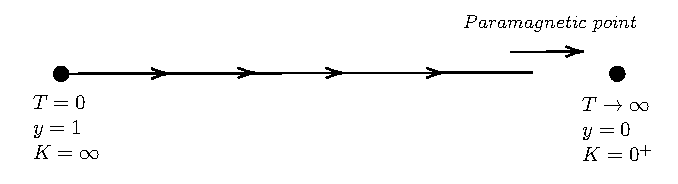
\includegraphics[width=0.8\textwidth]{../lessons/20_image/5.pdf}
\caption{\label{fig:20_5} One-dimensional flux of trajectories for Ising model for the recursion relation \( \tanh(K') = \tanh^2 (K) \). }
\end{figure}

\begin{remark}
For a generic scaling parameter \( l \) one can see that
\begin{equation*}
  \tanh K' = \qty( \tanh K )^l
\end{equation*}
Hence, we have
\begin{equation*}
  y' = y^l \quad l \ge 2
\end{equation*}
Therefore, the analysis for a scaling parameter \( l \ge 2 \) is similar to the \( l=2 \) case.
\end{remark}


\subsection{Decimation procedure for \( \pmb{d>1} \): proliferation of the interactions}
As we have stated, in \( d=1 \) the recursion relations can be determined without great problems and they don't introduce new interactions. However, this is not the case if \( d>1 \), and the value of the new coupling constants can't be determined exactly, forcing us to use approximations. Let us see with a generic example how the RG transformation can introduce new interactions in a two-dimensional Ising model with nearest-neighbour interactions.

Suppose we divide our system in blocks containing an odd number of spins and, similarly to what we have seen for \( d=1 \) in the previous sections, we sum over the spins on the boundary of the block and leave unchanged the one at the center.

We have problems with the spins at the boundaries. One can see that, in order to satisfy the condition
\begin{equation*}
  Z_N = Z_{N/l}
\end{equation*}
in addition to the parameters \( g' \) and \( K' \) at least one more interacting coupling must be considered

\begin{minipage}[c]{0.6\linewidth}
  \vspace{0.3cm}
Looking at the figure \ref{fig:20_6}, we see that the spin on the corder of the block 2 is coupled to one spin in bock 1 and one in block 3. When we sum over the spin in block 2 an effective coupling between blocks 1 and 3 will be established: we therefore see that the coarse-graining procedure introduces next-nearest-neighbour interactions between the blocks, so new terms are appearing in the Hamiltonian (which of course, as already stated, respect the symmetries of the original one):
\begin{equation*}
  \mathcal{H} \rightarrow \mathcal{H}' = \mathcal{H}' (K',K_2')
\end{equation*}
This unfortunately occurs at each iteration.
  \vspace{0.3cm}
\end{minipage}
\hspace{0.02\linewidth}
\begin{minipage}[]{0.35\linewidth}
\centering
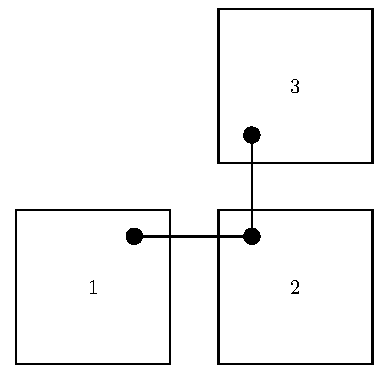
\includegraphics[width=1\textwidth]{../lessons/20_image/6.pdf}
\captionof{figure}{\label{fig:20_6}Introduction of a new effective interaction.}
\end{minipage}
Therefore, we understand that the iteration of the RG will introduce increasingly complicated couplings: this is the so called proliferation of interactions. In order to solve it, approximations are necessary.

\begin{figure}[h!]
\begin{minipage}[c]{0.5\linewidth}
\subfloat[][Square lattice. We sum over the red cross spins.]{ 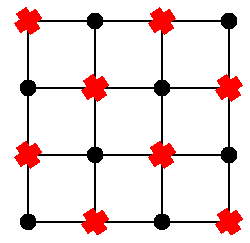
\includegraphics[width=0.8\textwidth]{../lessons/20_image/7.pdf}  \label{fig:20_7_1} }
\end{minipage}
\begin{minipage}[]{0.5\linewidth}
\centering
\subfloat[][New interactions introduced.]{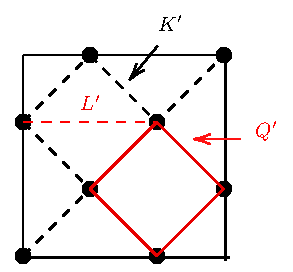
\includegraphics[width=0.8\textwidth]{../lessons/20_image/8.pdf}  \label{fig:20_7_2} }
\end{minipage}
\caption{\label{fig:20_7} Decimation for the two-dimensional Ising model with \( l=2 \).}
\end{figure}

\begin{example}{Decimation of Ising on square lattice}{}

  Let us now see in detail how to face the problem of the proliferation for a two-dimensional Ising model with nearest-neighbour interaction and \( H=0 \). We choose to coarse-grain the system summing over a "chessboard" of spins, as shown in Figure \ref{fig:20_7}. We call \( x \) the spin to sum over (red cross), while with \( o \) the other one (black circle).

The partition function in this case is:
\begin{equation*}
  Z_N (K,g) = \sum_{\{ o \}  }^{} \sum_{\{ x \}  }^{}   e^{\sum_{\expval{ij}
  }^{} w (S_i,S_j)  } = \sum_{\{ o \}  }^{} \sum_{\{ x \}  }^{}   e^{K \sum_{\expval{ij}}^{} S_i,S_j }
  =Z_{N/2} (K',L',Q',g')
\end{equation*}
By performing the sum and imposing the constraint \( Z_N  (K,g) = Z_{N/2} (K',L',Q',g') \), it is possible to show:
\begin{equation*}
  \begin{cases}
   k' = \frac{1}{4} \ln{\cosh 4 K} \\
   L' = \frac{1}{8} \ln{\cosh 4 K} \\
   Q' = \frac{1}{8} \ln{\cosh 4 K} - \frac{1}{2} \ln{\cosh 2 K}\\
  \end{cases}
\end{equation*}
This way, besides nearest-neighbour interactions (\( K \)) we are introducing also next-nearest-neighbour ones (\( K' \)  and \( L' \)) and also four-spin cluster interactions (\( Q' \)).
Note also that the final set of spins resides on a square whose side is \( \sqrt{2}  \)  times the original one, so we have that the scaling factor is \( l = \sqrt{2}  \).

If we now reiterate the procedure, more complicated interactions will appear and the problem becomes rapidly intractable. We therefore must do some approximations:

\begin{enumerate}

\item  We choose to neglect \( Q' \) (also because it is the only coupling that can become negative and thus prevent the spins from aligning).

\item Omit explicit dependence on \( L' \) defining a new constant \( K' \):
\begin{equation*}
   K'+L' \rightarrow K'
\end{equation*}
This way the recursion relation involves only \( K \).
\end{enumerate}
We end up with only one recursion:
\begin{equation*}
  K' = \frac{3}{8} \ln{\cosh 4 K}
\end{equation*}
Let us therefore see to which conclusions does this lead. The fixed points are given by:
\begin{equation*}
  K^* = \frac{3}{8} \ln{\cosh 4 K^*}
\end{equation*}
and the non-trivial (\( K^* \neq 0 \)) numerical solution of this equation is \( K_c=0.50698\dots \); the exact value found by Onsager is \( K_{exact}=
0.44069\dots \), so our approximation is good enough.
If we now set the initial value \( K_0 \), the we have:
\begin{equation*}
  \begin{cases}
   K^{(n)} \overset{n \rightarrow \infty }{\longrightarrow} \infty  & K_0 > K_c \\
   K^{(n)} \overset{n \rightarrow \infty }{\longrightarrow} 0  & K_0 < K_c
  \end{cases}
\end{equation*}
Thus, the fixed points \( K^*=0 \) and  \( K^* = \infty \)  are stable, while \( K^* = K_c \) is unstable; this can be visually represented as in Figure \ref{fig:20_8}


Let us now linearise the recursion relation near \( K_c \) and compute a couple of critical exponents.
On the base of what we have previously seen, if we call \( \delta K = K - K_c \) and \( \delta K' = K' - K_c \), we have:
\begin{equation*}
  \delta K' = \lambda _t \delta K = l^{y _t} \delta K
\end{equation*}
where
\begin{equation*}
  \lambda _t = \eval{\dv{K'}{K} }_{K=K_c}
\end{equation*}
Therefore, since also \( l = \sqrt{2}  \), we get:
\begin{equation*}
\begin{split}
y_t  &= \frac{\ln{\lambda _t} }{\ln{l} } = \frac{1}{\ln{\sqrt{2} } } \ln{\qty(\dv{K'}{K})_{K=K_c} }   \\
& = \frac{1}{\ln{\sqrt{2} } }  \ln{\qty(\dv{}{K} \qty(\frac{3}{8} \ln{(\cosh 4K)} ) ) } = 1.070\dots
\end{split}
\end{equation*}
it is positive, hence \( \lambda _t \)  is a relevant eigenvalue.
We have also the critical exponents:
\begin{equation*}
  \nu = \frac{1}{y_t} = 0.9345\dots, \qquad \alpha = 2 - \frac{d}{y_t} = 0.1313\dots
\end{equation*}
Onsager's exact result, as we know, gives \( \alpha =0 \) (since the specific heat diverges logarithmically, \( c_V = \ln t \)) and thus \( \nu =1 \). We therefore see that our approximation is sufficiently accurate (even if still improvable).

\end{example}



\begin{figure}[h!]
\centering
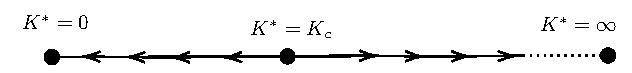
\includegraphics[width=0.6\textwidth]{../lessons/20_image/9.pdf}
\caption{\label{fig:20_8} RG flux of trajectories of the recursion relation \(   K^* = \frac{3}{8} \ln{\cosh 4 K^*} \). }
\end{figure}


\begin{figure}[h!]
\centering
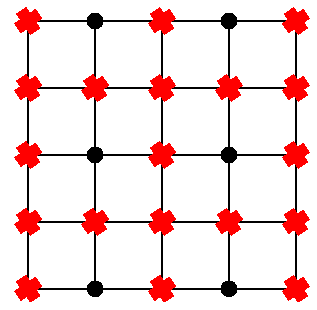
\includegraphics[width=0.37\textwidth]{../lessons/20_image/10.pdf}
\caption{\label{fig:20_9} Square lattice for the \( 2 \)-dimensional Ising model with \( l=2 \). The red cross are the spins to sum.}
\end{figure}


\subsubsection{Migdal-Kadanoff bond moving approximation}
The real-space renormalisation group can be performed exactly on the \( d=1 \)  Ising model by decimating a regular sequence of spins. This yields the following recursion relation for the coupling constant:
\begin{equation*}
  K' = \frac{1}{2} \ln \cosh (2K)
\end{equation*}
Unfortunately, this decimation can not be carried out exactly in higher dimensions and some truncation approximations are necessary.
One such scheme, which proved to be quite versatile is the so called Migdal-Kadanoff renormalisation (it is also called potential moving), which we illustrate here on the Ising model on the \( 2 \)-dimensional square lattice with \( l=2 \) defined in Figure \ref{fig:20_9}, where \( x \) are again the spin to sum over.

The idea is to remove the same interactions, i.e. same bonds; however a simple deletion of same bonds is a too strong approximation, therefore what we do is moving some bonds to neighbouring ones. In particular, we decimate every other line or column of spins along each lattice direction but removing the bonds not connected to the retained spins. Obviously, this simple approximation weakens the whole system, making it more “one-dimensional”. This is remedied by using the unwanted bonds to reinforce those that are left behind (see Figure \ref{fig:20_10}): the spins that are retained are now connected by a pair of double bonds of strength \( K \rightarrow 2K \).

\begin{figure}[h!]
\begin{minipage}[c]{0.5\linewidth}
\subfloat[][The original lattice. Some bonds are moved to neighbouring ones.]{ 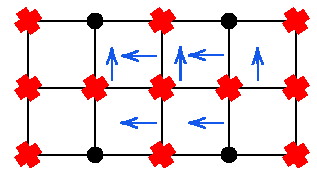
\includegraphics[width=0.8\textwidth]{../lessons/20_image/11.pdf}  \label{fig:} }
\end{minipage}
\begin{minipage}[]{0.5\linewidth}
\centering
\subfloat[][The lattice after the bonds moving step. The double bonds have coupling constant \( K \rightarrow 2K \). ]{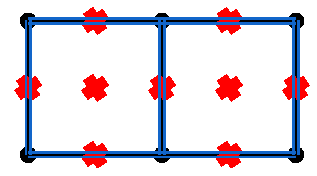
\includegraphics[width=0.8\textwidth]{../lessons/20_image/12.pdf}  \label{fig:} }
\end{minipage}
\caption{\label{fig:20_10} Migdal-Kadanoff for the Ising model on the square lattice with \( l=2 \).}
\end{figure}


After we have done this, the sum over \( x \) spins is similar to the Ising \( d=1 \) with \( l=2 \) and gives:
\begin{equation*}
  K' = \frac{1}{2} \ln \cosh (2 \vdot 2K)
\end{equation*}
where the crucial difference is the factor \( 2 \) in the \(\cosh (2 \vdot 2K)  \).
 The fixed point are given by:
\begin{equation*}
  K^* = \frac{1}{2} \ln \cosh (4 K^*)
\end{equation*}
Again we find \( K=0 \) and \( K= \infty  \)  fixed points:
\begin{itemize}
\item For \( K \gg 1 \) (\( T \rightarrow 0 \)):  unlike the \( d=1 \) we have \( K' \approx \frac{1}{2} \ln e^{4K} \approx 2K \) and hence the low temperature fixed point is also stable.
\item For \( K \ll 1 \) (\( T \rightarrow \infty  \)): we have \( K' \approx \frac{1}{2} \ln (1+16K^2) \approx 8K^2 \) so the high temperature fixed point is stable as it is in \( d=1 \).
\end{itemize}
Hence, in between we must have another unstable fixed point, which is given by:
\begin{equation*}
  e^{2K^*} = \frac{e^{4K^*} + e^{-4K^*}}{2} \quad \Rightarrow K^* = 0.305
\end{equation*}
Moreover, we have:
\begin{equation*}
  l^{y_t} = \eval{\dv{K'}{K} }_{K=K^*} \quad \Rightarrow y_t = 0.75
\end{equation*}
(remind that \( l=2 \)) while the exact solution is \( y_t = 1 \).

Comparing to the previous approximation, the Migdal-Kadanoff approximation gives a result further away from the true answer of \( K_c = 0.441 \). On the other hand, it is in a sense a more straightforward as the procedure did not generate any additional interactions.

This procedure is very easy to generalize in \( d \)-dimensions. For instance, if we consider an Ising cubic lattice (\( d=3 \)), we have three bonds to move, hence the coupling constant transforms as \( K \rightarrow 4K \). Generally, in \( d \)-dimensions, the coupling constant becomes:
\begin{equation*}
  K \rightarrow 2^{d-1}  K
\end{equation*}
Hence,
\begin{equation}
  K' = \frac{1}{2} \ln \cosh(2^{d-1} \vdot 2K)
\end{equation}
In conclusion, for a generic scaling factor \( l \), we have:
\begin{equation}
  K_l' = \frac{1}{2} \ln \cosh(l^{d-1} \vdot 2K)
\end{equation}
In higher dimensions the approximations worsens.

\subsection{Decimation procedure and transfer matrix method}
Let us consider the partition function
\begin{equation*}
  Z_N = \sum_{\{ S \}  }^{} \prod_{i=1}^{N} \overbrace{e^{w (S_i,S_{i+1})} }^{\bra{S_i} \mathbb{T} \ket{S_{i+1}}  }
  = \Tr(\mathbb{T}^N) =   \Tr(\mathbb{T}^2)^{N/2} = \Tr(\mathbb{T}^l)^{N/l}
\end{equation*}
Hence, after the renormalization procedure the transfer matrix transforms as:
\begin{equation}
  \mathbb{T}_l' = \mathbb{T}^l \quad \Rightarrow   \mathbb{T}_l' \qty( \{ K' \}  )  =   \mathbb{T} \qty(\{ K \}  )^l
  \label{eq:20_12}
\end{equation}
In the case in which the Migdal-Kadanoff approximation is considered, Eq.\eqref{eq:20_12} becomes
\begin{equation}
   \mathbb{T}_l' \qty( \{ K' \}  )  =   \mathbb{T} \qty(\{ l^{d-1} K \}  )^l
\end{equation}



\clearpage

\subsection{Migdal-Kadanoff for anysotropic Ising model on a square lattice}

Now, let us consider an anysotropic Ising model on a square lattice, as in Figure \ref{fig:20_11}. First of all, let us suppose that vertical bonds have \( K_y \equiv J_y/K_B T \), while horizontal ones \( K_x \equiv J_x/k_B T \). Hence, we have:
\begin{equation*}
  \frac{K_x}{K_y} = \frac{J_x}{J_y}
\end{equation*}

\begin{figure}[h!]
\centering
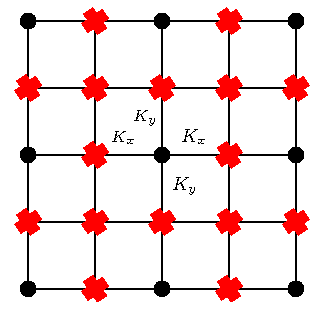
\includegraphics[width=0.35\textwidth]{../lessons/20_image/13.pdf}
\caption{\label{fig:20_11} Anysotropic Ising model on a square lattice, with coupling constants \( K_x \) and \( K_y \).}
\end{figure}



We proceed in the following way:
\begin{enumerate}
\item Firstly, we move the vertical bonds and double the ones that will survive, as in Figure \ref{fig:20_12_1}. The vertical bonds weight becomes:
\begin{equation*}
  K_y' = 2 K_y
\end{equation*}


\begin{figure}[h!]
\begin{minipage}[c]{0.5\linewidth}
\subfloat[][The lattice after the vertical bonds moving step.]{ 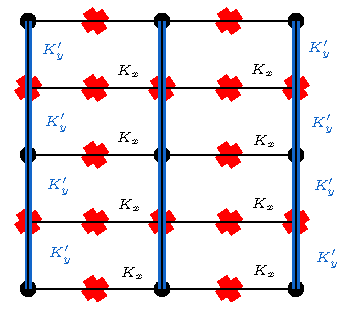
\includegraphics[width=0.8\textwidth]{../lessons/20_image/14.pdf}  \label{fig:20_12_1} }
\end{minipage}
\begin{minipage}[]{0.5\linewidth}
\centering
\subfloat[][The lattice after the vertical bonds moving step and after the sum of the spin along \( x \).]{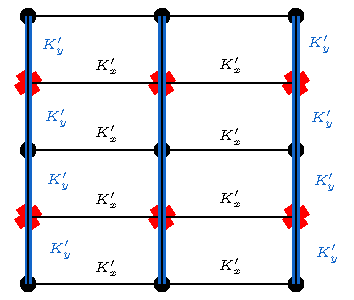
\includegraphics[width=0.8\textwidth]{../lessons/20_image/15.pdf}  \label{fig:20_12_2} }
\end{minipage}
\caption{\label{fig:20_12} }
\end{figure}

 We can now perform the sum of the spins, represented as a red cross in Fig.\ref{fig:20_12_1}, along the \( x \) direction as for the case \( d=1 \).
This gives
\begin{equation*}
  K_x' = \frac{1}{2} \ln \cosh (2K_x)
\end{equation*}
The lattice after this step is shown in Figure \ref{fig:20_12_2}.

\item We now perform the moving of the renormalized bonds \( K_x' \).
The bonds along \( x \) that survive will have weight
\begin{equation*}
  K_x'' = 2 K_x' = \ln \cosh (2K_x)
\end{equation*}
This step is illustrated in Figure \ref{fig:20_13}

\begin{figure}[h!]
\centering
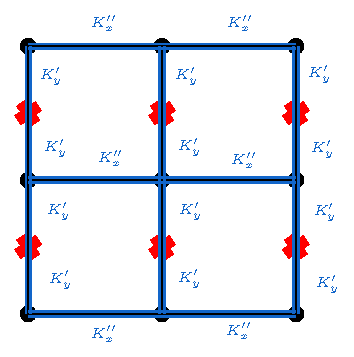
\includegraphics[width=0.4\textwidth]{../lessons/20_image/16.pdf}
\caption{\label{fig:20_13} The lattice after the renormalized horizontal bonds \( K_x' \)  moving step.}
\end{figure}



\item We finally perform the sum of the spins along the \( y \) direction as for the case \( d=1 \).
We obtain:
\begin{equation*}
  K_y'' = \frac{1}{2} \ln \cosh (2K_y') = \frac{1}{2} \cosh (4K_y)
\end{equation*}
The lattice after this step is shown in Figure \ref{fig:20_14}.

\begin{figure}[h!]
\centering
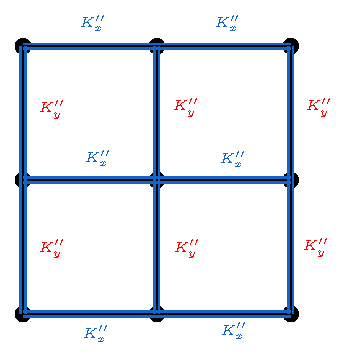
\includegraphics[width=0.4\textwidth]{../lessons/20_image/17.pdf}
\caption{\label{fig:20_14} The lattice after the sum of the spin along \( y \).}
\end{figure}

\end{enumerate}

The final recursion equations are:
\begin{equation}
  \begin{cases}
     K_x'' = 2 K_x' = \ln \cosh (2K_x) \\
       K_y'' = \frac{1}{2} \cosh (4K_y)
  \end{cases}
\end{equation}
Hence, the fixed points are given by:
\begin{equation}
  \begin{cases}
     K_x^* = \ln \cosh (2K_x^*) \\
       K_y^* = \frac{1}{2} \cosh (4K_y^*)
  \end{cases}
\end{equation}
Let us consider the case \( K_x = 2K_y \).
The couplings \( K_x \) and \( K_y \) at the fixed point are related by
\begin{equation}
  K_x^* = 2 K_y^*
\end{equation}
Hence, the value of \( K^* \) is \( (0.62,0.31) \). Moreover, we have:
\begin{subequations}
\begin{align*}
  \qty(\pdv{K_x''}{K_x} )_{K_x=K_x^*}  &=  2 \tanh 2K_x^* = 2^{y_t} \\
  \qty(\pdv{K_y''}{K_y} )_{K_y=K_y^*}  &=  2 \tanh 4K_y^* =  2 \tanh (2K_x^*) =2^{y_t}
\end{align*}
\end{subequations}
This gives \( y_t = 0.75 \). Let us note that \( y_t \) is the same as the one for the symmetric case.

\begin{figure}[h!]
\centering
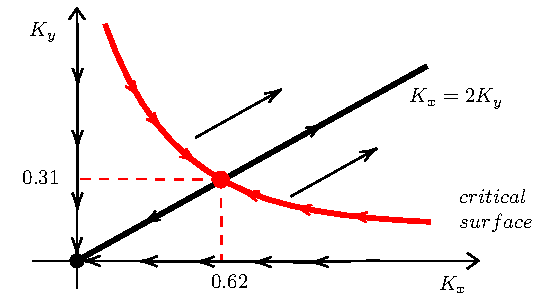
\includegraphics[width=0.7\textwidth]{../lessons/20_image/18.pdf}
\caption{\label{fig:20_15} \( (K_x,K_y) \) plane. The critical surface is represented in red, while the line \( K_x = 2 K_y \) in black. The intersection point is the critical point \( K^* = (0.62,0.31) \).  }
\end{figure}

Let us consider the plot in Figure \ref{fig:20_15}. We note that all points on the critical surface are critical with a given choice of \( K_x/K_y \). All these \( T_c (K_x/K_y) \) flow to the Ising model fixed point (same universality class).


\section{RG transformation: general approach}
A RG transformation reduces the number of degrees of freedom by \( l^d \), i.e. going from \( N \) to \( N' = N/l^d \).
This is achieved by performing a "partial trace" over the degrees of freedom, say, \( \{ S_i \}_1^N   \), and keeping the coarse grained degrees of freedom \( \{ S_I' \}_1^{N'}   \).
Formally, we can write (we call \( -\beta \mathcal{H} \rightarrow \mathcal{H}[K] \)):
\begin{equation}
  e^{\mathcal{H}_{N'}' \{ [K'],S_I' \}  } = \Tr_{\{ S_i \}  }' e^{ \mathcal{H}_N \{ [K],S_i \}  }  =
  \Tr_{\{ S_i \}  } P (S_i,S_I') e^{ \mathcal{H}_N \{ [K],S_i \}  }
\end{equation}
where \( \Tr'  \) is the constrained trace, while \( P (S_i,S_I')  \) is the \textbf{projection operator}, which "incorporates" the constraints and allows us to write an unconstrained trace. This operator must satisfy the following properties:
\begin{enumerate}

\item It must be built such that \( S_I' \) have the same range of values of \( S_i \) (i.e. if \( S_i = \pm 1 \), we should have \( S_I' = \pm1 \)).

\item \( P (S_i,S_I')\ge 0 \). This garantees that \( e^{\mathcal{H}_N' \{ [K'], S_I' \}  } \ge 0 \).

\item \( P (S_i, S_I') \) should preserve the symmetries of the original Hamiltonian.

\item \( \Tr_{\{ S_I' \}  } P (S_i,S_I') = \sum_{S_I'}^{}  P (S_i,S_I') = 1  \). This condition is necessary to satisfy
\begin{equation*}
  Z_{N'} [K'] = Z_N [K]
\end{equation*}
Indeed,
\begin{equation*}
\begin{split}
  Z_{N'} [K'] &= \Tr_{\{ S_I' \}  } e^{\mathcal{H}_{N'}' \{ [K'],S_I' \}  }
  = \Tr_{\{ S_I' \}  } \Tr_{\{ S_i \}  } P (S_i,S_{I}') e^{\mathcal{H}_N \{ [K],S_i \}  } \\
  & =  \Tr_{\{ S_i \}  }  \qty[ \Tr_{\{ S_I' \}  } P (S_i,S_I') ]   e^{\mathcal{H}_N \{ [K],S_i \}  }
   =  \Tr_{\{ S_i \}  }  e^{\mathcal{H}_N \{ [K],S_i \}  } \\ & = Z_N [K]
\end{split}
\end{equation*}

\end{enumerate}

In general this operator must be built "by hand". Let us see some examples.

\begin{example}{Block-Kadanoff transformation for \( \pmb{l=2} \)}{}
  For example, in the case of Kadanoff's block transformation we can assign the block spins \( S_I' \)  their values with the "majority rule", i.e. we build (hyper)cubic blocks of side \( (2l+1)a \) (so that each one contains an odd number of spins) and set:
\begin{equation*}
  S_I' = \text{sign} \qty(\sum_{i \in I}^{} S_i ) = \pm 1
\end{equation*}
and the projection operator can be written as:
\begin{equation*}
  P (S_i, S_I') = \prod_{I}^{}  \delta \qty(S_I' - \text{sign} \qty(\sum_{i \in I}^{} S_i  ) )
\end{equation*}
As we can see, doing an unconstrained trace with this operator is equivalent to performing the constrained trace.

\end{example}

\begin{example}{Decimation in \( \pmb{d=1} \) with \( \pmb{l=2} \)}{}
Let us do decimation in \( d=1 \) with \( l=2 \). In this case, \( S_I' \) are the even sites \( I=2i \). Hence, we have:
\begin{equation*}
  P (S_i, S_I') = \prod_{I=1}^{N/2} \delta \qty( S_I' - S_{2i})
\end{equation*}
The partition function is:
\begin{equation*}
\begin{split}
  Z_{N/2}' &= \Tr_{\{ S_i \}  } P (S_i, S_I') e^{\sum_{i}^{} w (S_{2i}, S_{2i+1}) }   \\
  &= \Tr_{\{ S_i \}  } \qty[ \prod_{I=1}^{N/2} \delta \qty( S_I' - S_{2i}) ]  e^{\sum_{i}^{} w (S_{2i}, S_{2i+1}) }  \\
  &= \Tr_{S_I'}   \prod_{I=1}^{N/2} \qty( \sum_{S_{2i+1} = \pm1}^{} e^{ w (S_I',S_{2i+1} ) + w (S_{2i+1}, S_{I+1}' )}   )
\end{split}
\end{equation*}


\end{example}

\subsection{Variational RG}
In this scheme the projection operator \( P(S_i,S_I') \) depends on a set of parameters \( \{ \lambda  \}   \) and the RG transformation is formally
\begin{equation*}
  e^{\mathcal{H}_{N'}' \{ [K'], \{ \lambda  \}, S_I'   \}  } = \Tr_{\{ S_i \}  } P (S_i,S_I', \{ \lambda  \}  ) e^{\mathcal{H}_N \{ [K], S_i \}  }
\end{equation*}
After choosing a certain form of \(  P (S_i,S_I', \{ \lambda  \}  ) \), one can minimize, over the space of \( \{ \lambda  \}   \), the expression:
\begin{equation*}
  \underbrace{ \log \qty(  \Tr_{\{ S_i \}  }   e^{\mathcal{H}_N \{ [K], S_i \}  } )  }_{\propto F_N}
  - \underbrace{\log \qty(  \Tr_{\{ S_I' \}  }   e^{\mathcal{H}_{N'}' \{ [K'], \{ \lambda  \}, S_I'   \}  }   )    }_{\propto F_{N'}}
\end{equation*}
Notice that, when
\begin{equation*}
   \Tr_{\{ S_I' \}  }  P (S_i,S_I', \{ \lambda  \}  ) = 1
\end{equation*}
the RG transformation is exact. In general, it is not possible to choose the parameters \(  \{ \lambda  \} \) to satisfy this condition and various schemes have been introduced to minimize
\begin{equation*}
  \Delta F = F_N - F_{N'}
\end{equation*}







\section{Real space renormalization group on 1D Ising model (H=0)}


\subsection{Decimation procedure for \( D=1 \)}
Decimation means summing up over all spins.
\( D=1 \) the procedure is clearly exact. Idea: pass from a \( N- \) spins system to one with \( \frac{N}{b} \) spins by summing the remaining \( N- \frac{N}{b} \) spins.


Case b=3 (see Figure \ref{fig:20_1}).

\begin{figure}[h!]
\centering
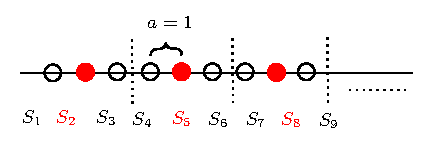
\includegraphics[width=0.6\textwidth]{../lessons/20_image/1.pdf}
\caption{\label{fig:20_1} Description.}
\end{figure}

Sum over the spins with the empty circle at the border of each clok, keeping the spins full circle untouched.
We obtain Figure \ref{fig:20_2}.

\begin{figure}[h!]
\centering
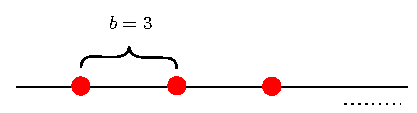
\includegraphics[width=0.6\textwidth]{../lessons/20_image/2.pdf}
\caption{\label{fig:20_2} Description.}
\end{figure}

Let us see how it works for the two blocks \( [S_1,S_2,S_3] \) and \( [S_4,S_5,S_6] \). Let us call
\begin{equation}
  S_2 \equiv S_1', \quad S_5 = S_2' \quad \text{fixed}
\end{equation}
\begin{equation}
  \sum_{S_3 = \pm 1}^{}   \sum_{S_4 = \pm 1}^{}  \exp [ k S_1' S_3 + k S_3 S_4 + k S_4 S_2']
\end{equation}
Since
\begin{equation}
  e^{k S_3 S_4}  = \cosh (k) ( 1 + x S_3 S_4)
\end{equation}
with
\begin{equation}
  x \equiv \tanh k
\end{equation}
we have
\begin{equation}
  \sum_{S_3,S_4}^{} \qty(\cosh k)^3 \qty(1 + x S_1' S_3) \qty(1 + x S_3 S_4) \qty(1 + x S_4 S_2')
\end{equation}
Performing the expansion and summing over \( S_3, S_4 \)  it is easy to show that (to do)
\begin{equation}
  Z_{N'}' (k') = \Tr_{ \{ S_I' \}  } \qty[ 2 ^{2N'} \qty( \cosh k)^{3N'} \qty(1 + x^3 S_I' S_{I+1} )  ]
  \label{eq:20_5}
\end{equation}
This must have the same form of \( Z_N (k) \). Hence, we should rewrite equation \eqref{eq:20_5} as
\begin{equation}
  Z_{N'}' (k') = \Tr_{ \{ S_I' \}  } \exp [ - \beta \mathcal{H}' (k')]
\end{equation}
with
\begin{equation}
  - \beta \mathcal{H}' = N' g (k,k') + k' \sum_{I}^{} S_I' S_{I+1}'
\end{equation}
We note that
\begin{equation}
\begin{split}
2^2 \qty(\cosh k)^3 (1 + x^3 S_I' S_{I+1}')   &=  2^2 \frac{\cosh k'}{\cosh k'}
 \qty(\cosh k)^3  (1 + x^3 S_I' S_{I+1}') \\
 & = 2^2 \frac{(\cosh k)^3}{\cosh k'}
  \qty(\cosh k')  (1 + x' S_I' S_{I+1}') \\
  & = 2^2 \frac{(\cosh k)^3}{\cosh k'}
   \exp (k' S_I' S_{I+1}') \\
   & = \exp [ 2 \ln{2} + \ln{ \qty[ \frac{(\cosh k)^3}{\cosh k'}] }  + k' S_I' S_{I+1}' ]
\end{split}
\end{equation}
It is ok with
\begin{equation}
  \begin{cases}
   g(k,k') = 2 \ln{2} +  \ln{ \qty[ \frac{(\cosh k)^3}{\cosh k'}] } \\
   x' = x^3  \iff k'= \tanh^{-1} \qty[ (\tanh k)^3] \Rightarrow k' = R_{b=3} (k)\\
   N' = \frac{N}{b}
  \end{cases}
\end{equation}
For \( x' = x^3 \), we have two fixed points
\begin{equation}
  \begin{cases}
   x^* = 0 \iff k \rightarrow 0 \iff T \rightarrow \infty \\
   x^* = 1^- \iff k \rightarrow \infty  \iff T \rightarrow 0
  \end{cases}
\end{equation}
For \( \forall x_0 < 1 \), we have \( R^{(n)} \overset{n \rightarrow \infty }{\longrightarrow} 0^+ \), \( x=1 \) is an unstable fixed point, as shown in Figure  \ref{fig:20_3}.
\begin{figure}[h!]
\centering
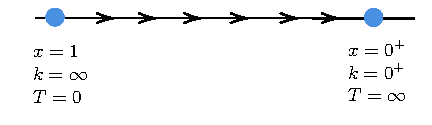
\includegraphics[width=0.6\textwidth]{../lessons/20_image/3.pdf}
\caption{\label{fig:20_3} Description.}
\end{figure}
We have
\begin{equation}
  \xi (x') = \frac{\xi (x)}{b}, \quad \text{with } x' = x^b
\end{equation}
where \( b \) is arbitrary. Let us choose \( b = c / \ln{x}  \):
\begin{equation}
  \xi (x^b) = \xi  \qty(e ^{b \ln{x} }) = \xi (e^c) = \frac{\xi (x)}{b}
  = \qty(\frac{c}{\ln{x} })^{-1} \xi (x)
\end{equation}
Finally,
\begin{equation}
  \xi (e^c) = \frac{\ln{x} }{c} \xi (x) \quad \Rightarrow \xi (x) = \frac{c \xi (e^c)}{\ln{x} } = \frac{const}{\ln{x} }
\end{equation}
\begin{equation}
  \xi (k) = \frac{const}{\ln{\qty(\tanh k) } }
\end{equation}
equal to the exact model in \( D=1 \).
\( k \rightarrow \infty  \) \( (x \rightarrow 1) \), we have
\begin{equation}
  \xi \sim e^{const/T}
\end{equation}
finite \( \forall k \neq \infty  \).









\end{document}
